\documentclass[11pt,twoside,a4paper]{book}
%\usepackage[portuguese,brazilian]{babel}
\usepackage[utf8]{inputenc}
\usepackage[T1]{fontenc}
\usepackage{latexsym}

\usepackage[brazil,brazilian]{babel}
\usepackage[pdftex]{graphicx}           
\usepackage{setspace}                   
\usepackage{indentfirst}                
\usepackage{makeidx}                  
\usepackage[nottoc]{tocbibind}     
\usepackage{courier}                    
\usepackage{type1cm}              
\usepackage{listings}                   
\usepackage{titletoc}
\usepackage{amsmath}
\usepackage[fixlanguage]{babelbib}
\usepackage[font=small,format=plain,labelfont=bf,up,textfont=it,up]{caption}
\usepackage[usenames,svgnames,dvipsnames]{xcolor}
\usepackage[a4paper,top=2.54cm,bottom=2.0cm,left=2.0cm,right=2.54cm]{geometry} % margens
\usepackage[pdftex,plainpages=false,pdfpagelabels,pagebackref,colorlinks=true,citecolor=DarkGreen,linkcolor=NavyBlue,urlcolor=DarkRed,filecolor=green,bookmarksopen=true]{hyperref} % links coloridos
\usepackage[all]{hypcap}                % soluciona o problema com o hyperref e capitulos
\usepackage[square,sort,nonamebreak,comma]{natbib}  
\usepackage[chapter]{algorithm}
\usepackage{algpseudocode}
\fontsize{60}{62}\usefont{OT1}{cmr}{m}{n}{\selectfont}
\usepackage{fancyhdr}
\pagestyle{fancy}
\fancyhf{}
\renewcommand{\chaptermark}[1]{\markboth{\MakeUppercase{#1}}{}}
\renewcommand{\sectionmark}[1]{\markright{\MakeUppercase{#1}}{}}
\renewcommand{\headrulewidth}{0pt}
\graphicspath{{imagens/}}             
\frenchspacing                          
\urlstyle{same}                         
\makeindex                              
\raggedbottom                           
\fontsize{60}{62}\usefont{OT1}{cmr}{m}{n}{\selectfont}
\cleardoublepage
\normalsize
% Ref: http://en.wikibooks.org/wiki/LaTeX/Packages/Listings
\lstset{ %
language=Java,                  % choose the language of the code
basicstyle=\footnotesize,       % the size of the fonts that are used for the code
numbers=left,                   % where to put the line-numbers
numberstyle=\footnotesize,      % the size of the fonts that are used for the line-numbers
stepnumber=1,                   % the step between two line-numbers. If it's 1 each line will be numbered
numbersep=5pt,                  % how far the line-numbers are from the code
showspaces=false,               % show spaces adding particular underscores
showstringspaces=false,         % underline spaces within strings
showtabs=false,                 % show tabs within strings adding particular underscores
frame=single,	                % adds a frame around the code
framerule=0.6pt,
tabsize=2,	                    % sets default tabsize to 2 spaces
captionpos=b,                   % sets the caption-position to bottom
breaklines=true,                % sets automatic line breaking
breakatwhitespace=false,        % sets if automatic breaks should only happen at whitespace
escapeinside={\%*}{*)},         % if you want to add a comment within your code
backgroundcolor=\color[rgb]{1.0,1.0,1.0}, % choose the background color.
rulecolor=\color[rgb]{0.8,0.8,0.8},
extendedchars=true,
xleftmargin=10pt,
xrightmargin=10pt,
framexleftmargin=10pt,
framexrightmargin=10pt
}

%----------------------------------------------
%\title{Uma infraestrutura para o desenvolvimento de aplicações distribuídas baseada em minitransações}
%\author{Leandro Ferro Luzia}
%\date{2012}
%-----------------------------------------------

% Corpo do texto
\begin{document}
\frontmatter 
\fancyhead[RO]{{\footnotesize\rightmark}\hspace{2em}\thepage}
\setcounter{tocdepth}{2}
\fancyhead[LE]{\thepage\hspace{2em}\footnotesize{\leftmark}}
\fancyhead[RE,LO]{}
\fancyhead[RO]{{\footnotesize\rightmark}\hspace{2em}\thepage}

\onehalfspacing

% ---------------------------------------------------------------------------- %
% CAPA
% Nota: O título para as dissertações/teses do IME-USP devem caber em um 
% orifício de 10,7cm de largura x 6,0cm de altura que há na capa fornecida pela SPG.
\thispagestyle{empty}
\begin{center}
    \vspace*{2.3cm}
    \textbf{\Large{Uma infraestrutura para desenvolvimento de aplicações distribuídas baseada em minitransações}}\\
    
    \vspace*{1.2cm}
    \Large{Leandro Ferro Luzia}
    
    \vskip 2cm
    \textsc{
    Dissertação apresentada\\[-0.25cm] 
    ao\\[-0.25cm]
    Instituto de Matemática e Estatística\\[-0.25cm]
    da\\[-0.25cm]
    Universidade de São Paulo\\[-0.25cm]
    para\\[-0.25cm]
    obtenção do título\\[-0.25cm]
    de\\[-0.25cm]
    Mestre em Ciências}
    
    \vskip 1.5cm
    Programa: Ciências da Computação\\
    Orientador: Prof. Dr. Francisco C. R. Reverbel
    \vskip 1cm
    
    \vskip 0.5cm
    \normalsize{São Paulo, Abril de 2012}
\end{center}

% ---------------------------------------------------------------------------- %
% Página de rosto (SÓ PARA A VERSÃO DEPOSITADA - ANTES DA DEFESA)
% Resolução CoPGr 5890 (20/12/2010)
\newpage
\thispagestyle{empty}
    \begin{center}
        \vspace*{2.3 cm}
        \textbf{\Large{Uma infraestrutura para desenvolvimento de aplicações distribuídas baseada em minitransações}}\\
        \vspace*{2 cm}
    \end{center}

    \vskip 2cm

    \begin{flushright}
	Esta é a versão original da dissertação elaborada pelo\\
	candidato Leandro Ferro Luzia, tal como \\
	submetida à Comissão Julgadora.
    \end{flushright}

\pagebreak

\pagenumbering{roman}

%\chapter*{Agradecimentos}
%Texto texto texto texto texto texto texto texto texto texto texto texto texto
%texto texto texto texto texto texto texto texto texto texto texto texto texto
%texto texto texto texto texto texto texto texto texto texto texto texto texto
%texto texto texto texto. Texto opcional.

\chapter*{Resumo}

\noindent LUZIA, L. F. \textbf{Uma infraestrutura para desenvolvimento de aplicações distribuídas baseada em minitransações}. 
2012. 120 f.
Dissertação (Mestrado) - Instituto de Matemática e Estatística,
Universidade de São Paulo, São Paulo, 2012.
\\

A proposta deste trabalho é implementar uma infraestrutura para sistemas distribuídos que possibilite o compartilhamento de estado entre as máquinas do sistema utilizando minitransações. As minitransações são uma modificação do protocolo de efetivação de duas fases em que todas as operações que compõem a transação são enviadas de uma só vez, diminuindo o custo de comunicação entre as máquinas do sistema. Através do uso da primitiva de minitransação os desenvolvedores podem projetar sistemas distribuídos baseando o compartilhamento de estado entre as máquinas em estruturas de dados, e não na troca explícita de mensagens. As máquinas terão à disposição um repositório de dados que pode crescer de forma a acomodar grandes quantidades de dados e que permite que aplicações tenham sempre acesso a dados consistentes. Assim, esperamos que o desenvolvimento da aplicação distribuída seja mais simples e ajude o desenvolvedor a focar nas necessidades reais da aplicação.
\\

\noindent \textbf{Palavras-chave:} minitransação, transação, banco de dado, sistemas distribuídos.

\chapter*{Abstract}
\noindent LUZIA, L. F. \textbf{An infrastructure for developing distributed applications based in minitransactions}. 
2010. 120 f.
Dissertação (Mestrado) - Instituto de Matemática e Estatística,
Universidade de São Paulo, São Paulo, 2012.
\\

The proposal of this work is to implement a distributed systems infrastructure that allows state sharing among system machines using minitransactions. Minitransactions are a modification in two phase commit protocol such that all transaction operations are sent in one network round trip, reducing the overhead of communication. By using the mintransaction primitive developers can design distributed systems in which the state sharing is based in the usage of data structures and not explicit message exchange. The machines will have access to a data repository that can grow to serve large amounts of data and allow applications to always access consistent data. That way, we hope that the distributed application development may became simpler and help developers to focus in the real needs of the applications.
\\

\noindent \textbf{Keywords:} minitransaction, transaction, database, distributed systems.

\tableofcontents

\chapter{Lista de Abreviaturas}
\begin{tabular}{ll}
	ACID    & Atomicidade, Consistência, Isolamento e Durabilidade \\
            & (\emph{Atomicity, Consistency, Isolation and Durability})\\
    SGBD	& Sistema Gerenciador de Banco de Dados\\
	2PC		& Efetivação em Duas Fases (\emph{Two-Phase Commit})\\
	TCP/IP	& Conjunto de protocolos de comunicação utilizado na Internet\\
			& (\emph{Transmition Control Protocol} e \emph{Internet Protocol})\\
\end{tabular}

\listoffigures
\listoftables
\listofalgorithms

\mainmatter

% cabeçalho para as páginas de todos os capítulos
\fancyhead[RE,LO]{\thesection}

\singlespacing              % espaçamento simples

\chapter{Introdução}
\label{chap:introducao}
Há diversos motivos para construir uma aplicação de forma distribuída --- compartilhamento de recursos (permitir o acesso a recursos específicos, como impressoras), tolerância a falhas (adicionando mais máquinas ao sistema aumenta a chance de que, a qualquer momento, haja pelo menos uma máquina capaz de responder pelo sistema) e escalabilidade (particionar e distribuir a carga de processamento do sistema permite que este suporte um número crescente de usuários e informações) são alguns deles.

Embora o compartilhamento de recursos e dados, tolerância a falhas parciais do sistema e aumento da disponibilidade sejam características altamente desejáveis de um sistema, tornar operante um sistema distribuído com estas características pode ser difícil. Diferentes plataformas de máquinas e diferentes sistemas operacionais, comunicação não síncrona entre as máquinas, conhecimento de cada máquina sobre as informações do sistema limitado aos dados locais e falhas parciais das máquinas fazem com que o desenvolvimento de aplicações distribuídas exija um esforço adicional em relação a sistemas convencionais.

De forma geral, um sistema distribuído é uma coleção de dispositivos computacionais individuais que podem comunicar-se uns com os outros \cite{tanenbaum, distributed_computing}. Essa definição engloba uma gama de sistemas computacionais atuais, desde placas de circutos integrados contendo diversos processadores até a \emph{internet}. Os sistemas distribuídos a que este trabalho se refere situam-se mais próximos da internet, sendo constituídos por diversos computadores interligados por uma rede de comunicação. Nestes sistemas, cada processador tem acesso somente ao seu próprio sistema de armazenamento (memória e disco), e a única forma de compartilharem informação é através da troca de dados por uma rede de comunicação ou seja (modelo de comunicação é baseado na troca de mensagens, e não em memória compartilhada ***TODO colocar alguma referência que cite a diferença entre estes dois modelos....

Implementar o compartilhamento de estado da aplicação (o conjunto de informações que define o funcionamento do sistema) utilizando a troca de dados na rede não é trivial, em especial quando os dados possuem restrições semânticas que precisam ser mantidas e validadas. Se considerarmos o exemplo clássico de um sistema bancário em que as contas dos usuários estão distribuídas entre diversas máquinas e uma solicitação de transferência entre contas que estão em duas máquinas diferentes seja feita, é esperado que esta transferência subtraia uma certa quantia da conta de origem e adicione esta quantia na conta de destino, sem alterar o valor total das contas envolvidas. Se a máquina em que a conta de destino estiver falhar, a quantia subtraída da conta de origem deve ser reposta.

O problema descrito acima exige que as operações efetuadas em cada máquina --- subtrair uma quantia da conta de origem e adicionar essa quantia na conta de destino --- sejam consideradas como uma operação única em que ou as duas operações são bem sucedidas, ou nenhuma das duas irá ocorrer. Uma maneira de se garantir esta execução é através da utilização do protocolo \emph{2PC}. Este protocolo permite a coordenação da execução de operações em diversas máquinas e garante que todas as operações em todas as máquinas serão efetivadas somente se todas as máquinas concordarem com a efetivação. Ele basicamente efetua uma rodada de votação entre as máquinas para verificar a possibilidade da efetivação das operações, e uma rodada de notificação, em que as máquinas são notificadas do resultado da votação. As rodadas de votação e notificação ocorrem após a execução das operações, gerando mais mensagens na rede.

As minitransações são baseadas no protocolo \emph{2PC} --- há duas rodadas de mensagens, porém as operações para serem executadas são embutidas na própria mensagem da rodada de votação. Na primeira rodada, equivalente à votação do \emph{2PC}, as mensagens possuem basicamente três tipos de operações: comparação, leitura e escrita. A operação de comparação é essencial para as minitransações, uma vez que elas determinam o voto da máquina em relação à efetivar ou não. Caso a comparação seja bem sucedida, as escritas serão efetuadas e as leituras serão retornadas como resposta, e a máquina votará para efetivar as operações. Caso contrário nenhum dado será retornado, nenhuma escrita será efetuada e a máquina votará pela não efetivação das operações, causando o cancelamento da transação.

\section{Objetivo}
\label{sec:objetivo}
A proposta deste trabalho é implementar uma infraestrutura para sistemas distribuídos que possibilite o compartilhamento de estado entre as máquinas do sistema utilizando minitransações. Ao invés de trocarem mensagens explicitamente, as máquinas verão um repositório que pode crescer de forma a acomodar grandes quantidades de dados e que permite que todas as máquinas tenham sempre acesso a dados consistentes. Assim, esperamos que o desenvolvimento da aplicação distribuída seja mais simples e ajude o desenvolvedor a focar nas necessidades reais da aplicação.

Esta infraestrutura será composta por máquinas que formam o repositório de dados e implementam o protocolo de minitransações. O acesso a essas máquinas será feito pela rede, através da utilização de um protocolo simples da camada de aplicação TCP/IP, de forma a possibilitar que qualquer sistema que implemente o protocolo TCP/IP possa utilizar a infraestrutura.

\section{Organização do texto}
\label{sec:organizacao_do_texto}
Esta introdução apresenta o contexto de utilização das minitransações e os objetivos deste trabalho. O capítulo \ref{chap:conceitos} inicia com uma revisão sobre transações e sua utilidade, uma revisão do conceito de transações distribuídas e explica em detalhes o protocolo 2PC, ponto de partida para a derivação do procolo de minitransações. O capítulo \ref{chap:implementacao} apresenta a implementação da infraestrutura e detalha sua arquitetura (divisão de seus componentes) e os algoritmos e protocolos de execução das minitransações. O capítulo \ref{chap:cronograma} apresenta o andamento do trabalho e as expectativas em relação a datas para o término do trabalho.

\chapter{Conceitos}
\label{chap:conceitos}
Como as minitransações são uma extensão do protocolo 2PC, este capítulo irá apresentar uma revisão dos conceitos relacionados a transações, transações distribuídas e, por fim, uma detalhada explicação sobre as minitransações.

\section{Transações}
\label{sec:transacoes}
Aplicações executam operações, de variados tipos e para diversas finalidades, como somar dois números, ler uma tecla digitada do teclado ou enviar um \emph{email} através da rede. Vamos considerar por exemplo o algoritmo descrito em \ref{alg:transferencia_valores_sem_transacao}, que implementa a transferência de valores entre duas contas, origem e destino. Digamos que as funções $Ler$ e $Escrever$ implementam as operações de leitura e escrita em um gerenciador de recursos que armazene os dados das contas. Estas operações executam imediatamente e abortam a execução do programa caso algum erro ocorra.

O algoritmo irá obter uma referência às contas, verificar se o saldo da conta de origem é suficiente, subtrair o valor da conta de origem, somar este mesmo valor na conta de destino e escrever os novos valores nos recursos correspondentes. Se um erro ocorrer ao executar a escrita do novo valor na conta de destino os dados ficarão inconsistentes, pois o valor terá sido retirado da conta de origem ($Escrever(O, VO - V)$ já aconteceu), mas não terá sido adicionado à conta de destino ($Escrever(D, VD + V)$ falhou).

\begin{algorithm}
\caption{Transferência de valores}
\label{alg:transferencia_valores_sem_transacao}
\begin{algorithmic}[1]
\State $O \gets \text{ Recurso referente à conta de origem}$
\State $D \gets \text{ Recurso referente à conta de destino}$
\State $V \gets \text{ Valor a ser transferido}$
\State $VO \gets Ler(O)$
\If{$VO >= V$}
    \State $VD \gets Ler(D)$
    \State $Escrever(O, VO - V)$
    \State $Escrever(D, VD + V)$
\EndIf
\end{algorithmic}
\end{algorithm}

Como alternativa poderíamos fazer com que as funções $Ler$ e $Escrever$ não abortassem o programa caso algum erro ocorra, e que tivéssemos acesso a uma função, $HouveErro()$, pode ser usada para checar se a última operação $Ler$ ou $Escrever$ falhou. Assim, poderíamos implementar uma nova versão do algoritmo para transferência (algoritmo \ref{alg:transferencia_valores_checar_erro}).

\begin{algorithm}
\caption{Transferência de valores - verificação de erro}
\label{alg:transferencia_valores_checar_erro}
\begin{algorithmic}[1]
\State $O \gets \text{ Recurso referente à conta de origem}$
\State $D \gets \text{ Recurso referente à conta de destino}$
\State $V \gets \text{ Valor a ser transferido}$
\State $VO \gets Ler(O)$
\If{$VO >= V$}
    \State $VD \gets Ler(D)$
    \State $Escrever(O, VO - V)$
    \If{$HouveErro()$}
        \State $Imprimir($ERRO - não foi possível debitar valor$)$
    \Else
        \State $Escrever(D, VD + V)$
        \If{$HouveErro()$}
            \State $Escrever(O, VO + V)$
            \If{$HouveErro()$}
                \State $Imprimir($ERRO - dados ficarão inconsistentes!$)$
            \EndIf
        \EndIf
    \EndIf
\EndIf
\end{algorithmic}
\end{algorithm}

Como podemos ver, as operações que precisam ser desfeitas caso algum erro ocorra são operações de escrita, ou de forma mais geral, operações que alteram o estado do sistema. Apesar de o procedimento de correção no algoritmo \ref{alg:transferencia_valores_checar_erro} ser simples, à medida que o número de alterações efetuadas aumenta, a complexidade do procedimento de correção aumenta também. Se tivéssemos três contas envolvidas, uma de origem e duas de destino, o procedimento ficaria mais complicado, como podemos ver no algoritmo \ref{alg:transferencia_valores_tres_contas}, em que o valor subtraído da conta de origem é igualmente divido entre as contas de destino 1 e 2.

\begin{algorithm}
\caption{Transferência de valores - complexidade na correção de erros}
\label{alg:transferencia_valores_tres_contas}
\begin{algorithmic}[1]
\State $O \gets \text{ Recurso referente à conta de origem}$
\State $D_1 \gets \text{ Recurso referente à conta de destino 1}$
\State $D_2 \gets \text{ Recurso referente à conta de destino 2}$
\State $V \gets \text{ Valor a ser transferido}$
\State $VO \gets Ler(O)$
\If{$VO >= V$}
    \State $VD_1 \gets Ler(D_1)$
    \State $VD_2 \gets Ler(D_2)$
    \State $Escrever(O, VO - V)$
    \If{$HouveErro()$}
        \State $Imprimir($ERRO - não foi possível debitar valor$)$
    \Else
        \State $Escrever(D_1, VD_1 + V/2)$
        \If{$HouveErro()$}
            \State $Escrever(O, VO + V)$
            \If{$HouveErro()$}
                \State $Imprimir($ERRO - dados ficarão inconsistentes!$)$
            \EndIf
        \Else
            \State $Escrever(D_2, VD_2 + V/2)$
            \If{$HouveErro()$}
                \State $Escrever(O, VO + V)$
                \If{$HouveErro()$}
                    \State $Imprimir($ERRO - dados ficarão inconsistentes!$)$
                \EndIf
                \State $Escrever(D_1, VD_1 - V/2)$
                \If{$HouveErro()$}
                    \State $Imprimir($ERRO - dados ficarão inconsistentes!$)$
                \EndIf
            \EndIf
        \EndIf
    \EndIf
\EndIf
\end{algorithmic}
\end{algorithm}

Este complexo tratamento de erros, necessário para manter o estado do sistema consistente, é resultado do fato que as operações de leitura e escrita dos algoritmos fazem parte de uma operação lógica mais abrangente, a transferência de valores, que só pode ocorrer por completo caso todas as operações que a constituem sejam executadas corretamente. Esta operação lógica constituída por um conjunto de operações sobre os recursos do sistema é chamada de \textbf{transação}. O uso mais clássico e difundido de transações é feito na área de banco de dados, em que uma transação é a unidade de execução de operações, composta por uma sequência de comandos de leitura e escrita de dados \cite{garcia-molina, vaca}.

O uso de transações para o desenvolvimento de aplicativos facilita a maneira como o aplicativo pode ser implementado. Por exemplo, digamos que a transferência de valores do algoritmo \ref{alg:transferencia_valores_tres_contas} possa ser agora implementada utilizando um gerenciador de recursos que suporte o agrupamento de operações em uma transação, como no algoritmo \ref{alg:transferencia_valores_transacao}. Neste algoritmo introduzimos três novas funções: $IniciarTransacao$, para criar uma nova transação, retornando um identificador para a transação criada; $Efetivar(T)$, que sinaliza que as alterações efetuadas pela transação $T$ podem ser realmente executadas; e $Abortar(T)$, que indica que a transação foi cancelada e que alterações por ela efetuadas não surtirão efetio. As operações $Ler$ e $Escrever$ foram alteradas para referenciar a transação da qual fazem parte.

\begin{algorithm}
\caption{Transferência de valores - uso de transações}
\label{alg:transferencia_valores_transacao}
\begin{algorithmic}[1]
\State $O \gets \text{ Arquivo referente à conta de origem}$
\State $D_1 \gets \text{ Arquivo referente à conta de destino 1}$
\State $D_2 \gets \text{ Arquivo referente à conta de destino 2}$
\State $V \gets \text{ Valor a ser transferido}$
\State $T \gets IniciarTransacao()$
\State $VO \gets Ler(T, O)$
\If{$VO >= V$}
    \State $VD_1 \gets Ler(T, D_1)$
    \State $VD_2 \gets Ler(T, D_2)$
    \State $Escrever(T, O, VO - V)$
    \State $E_1 \gets HouveErro()$
    \State $Escrever(T, D_1, VD_1 + V/2)$
    \State $E_2 \gets HouveErro()$
    \State $Escrever(T, D_2, VD_2 + V/2)$
    \State $E_3 \gets HouveErro()$
    \If{$E_1 \wedge E_2 \wedge E_3$}
        \State $Abortar(T)$
    \Else
        \State $Efetivar(T)$
    \EndIf
\EndIf
\end{algorithmic}
\end{algorithm}

Da mesma maneira que as transações são utilizadas para garantir a consistência dos dados em casos de falha na execução de operações, elas podem ser utilizadas também no caso de falhas da própria aplicação. Vamos supor que, por algum motivo, a aplicação executando o algoritmo \ref{alg:transferencia_valores_transacao} seja cancelada, deixando de executar entre as linhas 10 e 11. O valor será subtraído da conta de origem mas não será adicionado nas contas de destino. Neste caso, o sistema de arquivos poderia ele mesmo efetuar a operação $Abortar(T)$ para toda transação $T$ que esteja inativa por mais do que um determinado tempo.

Através do uso de uma transação a utilização dos recursos fica mais sucinta e as ações necessárias para abortar uma transação (desfazer as alterações) ou efetivá-la ficam a cargo do gerenciador de recursos utilizado. Para possibilitar que as alterações somente tenham efeito quando a transação for realmente efetivada ou que transações incompletas sejam descartadas, é utilizado, em geral, um registro de operações chamado \emph{log}. Este \emph{log} registra as alterações efetuadas pelas transações e deve ser gravado em um meio de armazenamento não volátil, como o disco rígido, para garantir que o gerenciador de recursos possa recuperar informações acerca das transações em caso de falhas.

Mesmo que a execução do algoritmo \ref{alg:transferencia_valores_transacao} deixe o sistema em um estado consistente, a execução concorrente deste algoritmo pode deixar o sistema em um estado inconsistente. Considere um cenário em que a conta A com o valor 20, as contas B, C, D e E com valor 0, uma aplicação tentando executar a transferência de 10 da conta A para as contas B e C, e uma outra aplicação tentando executar a transferência de 14 da conta A para as contas D e E. Se as duas aplicações efetuarem a verificação $VO >= V$ ao mesmo tempo, as duas verão o mesmo valor de $VO$ (20) e as duas irão executar a transferência (pois $V$ será 10 para uma e 14 para outra). Neste caso, o valor final de $VO$ pode ser tanto 10 quanto 6, dependendo de qual transação executar por último, B e C terão o valor 5 e D e E terão o valor 7. O valor total entre as contas não pode ser modificado por uma transferência, e neste caso vemos que antes da transferência tínhamos o valor 20 e depois temos o valor 34 ou 30, deixando o sistema com dados incorretos.

Para evitar que este tipo de problema ocorra, um gerenciador de recursos que possibilite a execução de transações concorrentes deve executar as operações de cada transação de uma maneira que uma transação não atrapalhe a execução de outra. Um \textbf{escalonamento} é uma sequência ordenada no tempo de operações de uma ou mais transações. Dois possíveis escalonamentos para as operações das transações do algoritmo \ref{alg:transferencia_valores_sem_transacao} podem ser vistos na tabela \ref{tab:exemplo_escalonamento}. Um \textbf{escalonamento sequencial} é um escalonamento em que as operações de uma transação estão agrupadas, ou seja, as operações de transações diferentes não são intercaladas, como pode ser visto na tabela \ref{tab:escalonamento_sequencial}, e um \textbf{escalonamento sequenciável} é um escalonamento em que o resultado de sua execução é equivalente ao resultado de uma execução de um escalonamento sequencial. O escalonamento ilustrado na tabela \ref{tab:escalonamento_sequenciavel} produz como resultado de sua execução o mesmo resultado da execução do escalonamento da coluna esquerda da tabela \ref{tab:escalonamento_sequencial}. O método tradicional para obter um escalonamento sequenciável é através do uso de \textbf{travas} associadas aos recursos acessados, de forma que um recurso só possa ser acessado se uma trava for obtida antes, e uma trava só pode ser obtida caso não haja nenhuma outra trava associada ao recurso.

Na literatura é utilizada a sigla \emph{ACID} (\textbf{A}tomicidade, \textbf{C}onsistência, \textbf{I}solamento e \textbf{D}urabilidade) para descrever as quatro propriedades que uma transação deve ter para que os requisitos descritos acima sejam atendidos:

\begin{enumerate}
\item \emph{Atomicidade}: ou todas as operações são executadas com sucesso, ou nenhuma operação é executada. Com isso, o desenvolvedor de aplicações não precisa se preocupar com o efeito de transações incompletas, como quando ocorrem falhas do sistema. %Esta propriedade é obtida através do desfazimento de operações já executadas de transações que não foram efetivadas. O gerenciador do banco de dados utiliza uma técnica em que as operações são primeiro escritas em uma tabela de registro de operações (\emph{log}), para depois serem efetivadas no banco de dados propriamente dito.
\item \emph{Consistência}: cada transação deve levar o banco de dados de um estado consistente para outro estado consistente. Esta propriedade depende essencialmente do desenvolvedor de aplicações e da semântica dos dados envolvidos. % ---o gerenciador de banco de dados pode auxiliar através de restrições sobre os dados que podem ser configuradas mas, no final, a semântica da consistência fica sob responsabilidade do desenvolvedor. %Se retomarmos ao exemplo do sistema bancário, a transferência entre as contas não deve alterar o valor total da soma dos saldos das contas individuais envolvidas na transação.
\item \emph{Isolamento}: a execução de uma transação não pode interferir na execução de outras transações, garantindo que mesmo que as operações executadas por diferentes transações possam ser intercaladas por questões de performance ou aproveitamento de recursos o resultado final da execução das transações será equivalente ao resultado de alguma execução sequencial de todas as transações.
\item \emph{Durabilidade}: uma vez que a transação tenha sido efetivada, os efeitos de sua execução devem persistir mesmo em casos de falha. A durabilidade garante que os efeitos gerados por uma transação efetivada sejam permanentes, mesmo que ocorram falhas após a efetivação da transação. %Um \emph{log} também é utilizado para a garantir a durabilidade. Uma vez que ocorra uma falha e o sistema se recupere, o gerenciador irá vasculhar o \emph{log} em busca de transações que tenham sido efetivadas mas cujos efeitos não estejam refletidos no banco de dados, para executar novamente os comandos da transação.
\end{enumerate}

%Estas quatro propriedades são conhecidas como propriedades \emph{ACID}. As transações \emph{ACID}, como são chamadas, são uma característica dos \emph{SGBD}s, permitindo que um grande número de aplicações utilizem de forma concorrente o banco de dados. Através da utilização destas transações uma aplicação pode interagir com o banco de dados sem notar que outras aplicações estão interagindo com o banco de dados também, acessando e alterando possivelmente os mesmos dados.

%A exposição de uma interface de acesso a um sistema através de transações \emph{ACID} (\textbf{A}tomicidade, \textbf{C}onsistência, \textbf{I}solamento e \textbf{D}urabilidade) permite que o desenvolvedor que utiliza este sistema pode utilizá-lo de mais simples e intuitiva, sem precisar se preocupar com controles de concorrência ou outros aspectos do tipo. Por exemplo, vamos supor que em um sistema de controle de contas bancárias existam três contas A, B e C com saldos 20, 10 e 5, respectivamente. Vamos considerar o algoritmo \ref{alg:transferencia_valores} que descreve a operação de transferência entre duas contas, origem e destino, de um determinado valor.

% \begin{algorithm}
% \caption{Transferência de valores entre contas}
% \label{alg:transferencia_valores}
% \begin{algorithmic}[1]
% \State $O \gets \text{ Conta de origem}$
% \State $D \gets \text{ Conta de destino}$
% \State $V \gets \text{ Valor a ser transferido}$
% \State $VO \gets Ler(O)$
% \If{$VO >= V$}
% 	\State $VD \gets Ler(D)$
% 	\State $Escrever(O, VO - V)$
% 	\State $Escrever(D, VD + V)$
% \EndIf
% \end{algorithmic}
% \end{algorithm}

% As funções $Ler$ e $Escrever$ representam as operações de leitura e escrita, respectivamente. Este algoritmo obtém o valor do saldo da conta de origem, verifica se este valor é maior que o valor a ser transferido e, caso seja maior, transfere o valor, somando a quantia ao valor de destino e subtraindo do valor de origem. Este algoritmo, portanto, garante que o valor da conta de origem nunca seja menor do que 0 e garante também que o valor subtraído da conta de origem seja somado ao valor da conta de destino, ou seja, o valor total das contas é o mesmo antes e depois da execução do algoritmo: $(VO - V) + (VD + V) = VO + VD$. Assumimos que o banco de dados neste exemplo considere cada execução de uma operação de forma independente, sem agrupá-las em uma operação lógica (transação).

% Embora este algoritmo esteja correto, se considerarmos a execução concorrente de aplicações que implementem este algoritmo poderemos observar eventuais inconsistências na invariante do sistema que diz que o valor total das contas deve ser mantido. Duas aplicações, que implementam este algoritmo, executando concorrentemente tentarão transferir, respectivamente, o valor 10 da conta A para a conta B e o valor 15 da conta A para a conta C. Como o banco de dados em questão não agrupa as operações em unidades lógicas, estas operações podem ser intercaladas de tal forma que as aplicações executem $VO \gets Ler(O)$ e observem o mesmo valor de $VO$. Como o valor inicial da conta A é 20, a condição $VO >= V$ será verdadeira para a duas aplicações (pois V será 10 para uma aplicação e 15 para outra) e, assim, as duas aplicações executarão a transferência e teremos então a conta B com saldo 20, a conta C com saldo 20 e a conta A poderá ter tanto o valor 10 quanto o valor 5 (dependendo de qual aplicação executar a escrita por último), totalizando 50 ou 45, ambos diferentes do valor inicial 35 (20 + 10 + 5).

% O fato de não agruparmos as operações em transações também dificulta o tratamento e a recuperação de erros. Se uma das aplicações em questão falhasse após a execução de $Escrever(O, VO - V)$ e antes de $Escrever(D, VD + V)$ os dados ficariam inconsistentes pois a quantia $V$ seria retirada de uma conta mas não seria adicionada à outra. Em um cenário deste tipo, o tratamento de insconsistências e recuperação de falhas deve ser feito por algum procedimento externo, como alguma aplicação especializada ou mesmo de forma manual, uma vez que, para o banco de dados, se uma operação foi executada corretamente, não houve problema nenhum.

% Se agruparmos as operações que cada execução do algoritmo \ref{alg:transferencia_valores} efetua em uma transação *** TODO parei aqui...

% Portanto, interações de transações concorrentes podem levar o banco de dados a um estado inconsistente, mesmo que individualmente cada transação garanta a consistência dos dados. Assim, para garantir a consistência dos dados algum tipo de controle de concorrência deve ser feito para permitir que as operações das diversas transações possam ser executadas concorrentemente. Para formalizar o estudo de um mecanismo que permita a execução concorrente e consistente de transações é utilizado o conceito de \textbf{escalonamento}, que é uma sequência ordenada, de forma temporal, de operações ($Ler$ e $Escrever$) de uma ou mais transações. Dois possíveis escalonamentos para as operações das transações descritas anteriormente podem ser vistos na tabela \ref{tab:exemplo_escalonamento} (consideramos que o tempo aumenta conforme as operações são executadas da primeira para a última linha da tabela).

\begin{table}
\caption{Dois possíveis escalonamentos para as operações de transferência entre contas}
\label{tab:exemplo_escalonamento}
\centering
\begin{tabular}{ | l | l | }
	\hline
	$Ler_1(O)$&$Ler_2(O)$\\
	$Ler_1(D)$&$Ler_1(O)$\\
	$Escrever_1(O, VO - V)$&$Ler_1(D)$\\
	$Ler_2(O)$&$Escrever_1(O, VO - V)$\\
	$Escrever_1(D, VD + V)$&$Ler_2(D)$\\
	$Ler_2(D)$&$Escrever_2(O, VO - V)$\\
	$Escrever_2(O, VO - V)$&$Escrever_2(D, VD + V)$\\
	$Escrever_2(D, VD + V)$&$Escrever_1(D, VD + V)$\\
	\hline
\end{tabular}
\end{table}

\begin{table}
\caption{Escalonamentos sequenciais das operações de transferência entre contas}
\label{tab:escalonamento_sequencial}
\centering
\begin{tabular}{ | l | l | }
	\hline
	$Ler_1(O)$&$Ler_2(O)$\\
	$Ler_1(D)$&$Ler_2(D)$\\
	$Escrever_1(O, VO - V)$&$Escrever_2(O, VO - V)$\\
	$Escrever_1(D, VD + V)$&$Escrever_2(D, VD + V)$\\
	&\\
	$Ler_2(O)$&$Ler_1(O)$\\
	$Ler_2(D)$&$Ler_1(D)$\\
	$Escrever_2(O, VO - V)$&$Escrever_1(O, VO - V)$\\
	$Escrever_2(D, VD + V)$&$Escrever_1(D, VD + V)$\\
	\hline
\end{tabular}
\end{table}

\begin{table}
\caption{Escalonamento sequenciável das operações de transferência entre contas}
\label{tab:escalonamento_sequenciavel}
\centering
\begin{tabular}{ | l | }
	\hline
	$Ler_1(O)$\\
	$Ler_1(D)$\\
	$Escrever_1(O, VO - V)$\\
	$Ler_2(O)$\\
	$Escrever_1(D, VD + V)$\\
	$Ler_2(D)$\\
	$Escrever_2(O, VO - V)$\\
	$Escrever_2(D, VD + V)$\\
	\hline
\end{tabular}
\end{table}

% Um \textbf{escalonamento sequencial} é um escalonamento em que as operações de uma transação estão agrupadas, ou seja, as operações de transações diferentes não são intercaladas, como pode ser visto na tabela \ref{tab:escalonamento_sequencial}. Um \textbf{escalonamento sequenciável} é um escalonamento em que o resultado de sua execução é equivalente ao resultado de uma execução de um escalonamento sequencial. O escalonamento ilustrado na tabela \ref{tab:escalonamento_sequenciavel} produz como resultado de sua execução o mesmo resultado da execução do escalonamento da coluna esquerda da tabela \ref{tab:escalonamento_sequencial}.

% Através do agrupamento de operações em transações e de um escalonamento destas operações

%O uso de mecanismos como \textbf{travas} e \emph{logs} são uma maneira de implementar um escalonamento sequenciável de operações de transações simultâneas. As travas controlam o acesso aos dados e os \emph{logs} permitem que operações possam ser refeitas ou desfeitas, garantindo assim isolamento entre as operações de diferentes transações e atomicidade e durabilidade em cenários de falhas.

%A atomicidade e a durabilidade das transações é garantida através da utilização do \emph{log}, uma estrutura que registra as operações que alteram os dados do sistema em uso. O \emph{log} permite que alterações possam ser desfeitas em um cenário de falha de alguma operação, garantindo a atomicidade da transação; permite também que operações possam ser refeitas caso ocorra alguma falha entre a efetivação da transação e a escrita permanente 

%Um escalonamento sequenciável pode ser obtido através do uso de \textbf{travas} (\emph{locks}), um mecanismo que permite identificar quais dados estão sendo usados, e de que forma, para verificar se esses dados podem ser acessados para leituras ou escritas. A utilização de um escalonamento sequenciável aliada à utilização de um \emph{log} permite que 

%O tipo de trava mais simples é uma varíavel binária associada ao dado: caso essa variável tenha valor 0 o dado não está travado por outra transação e pode ser utilizado, atribuindo então o valor 1 a essa variável durante a utilização; caso o valor seja 1, o dado está sendo utilizado e não pode ser acessado até que o valor da variável seja 0. As transações precisam portanto adquirir travas para que possam ler ou escrever os dados, e precisam liberar estas travas ao fim da operação para permitir que outras transações possam utilizar os mesmos dados. Este tipo de trava binária é um tanto restritiva pois impede a ocorrência concorrente de operações que não causam inconsistência dos dados, como leituras concorrentes, e um tipo mais sofisticado será apresentado na seção \ref{chap:implementacao}.

%Travas são um exemplo de abordagem pessimista para controle de concorrência. Existe também a abordagem otimista, em que o gerenciador permite que os dados sejam alterados e acessados sem nenhum controle prévio. De forma simplificada, mecanismos que utilizam a abordagem otimista copiam os dados para uma área temporária exclusiva da transação, e as operações são efetuadas nesta área. Somente no momento da efetivação é que o gerenciador irá checar se houve conflito com outras transações, e então é necessário algum mecanismo para resolução destes conflitos. Como a implementação apresentada em \ref{chap:implementacao} irá utilizar uma abordagem pessimista, não iremos abordar este assunto a fundo.

%*** TODO verificar se vale a pensa citar os níveis de isolamento de transações... acho que vale, por que o uso de travas faz mais sentido para o nível READ COMMITED, que é o default, mas existem outros níveis mais "frouxos"...

\section{Transações distribuídas}
\label{sec:transacoes_distribuidas}
Bancos de dados distribuídos apresentam benefícios tais como a possibilidade de paralelização e melhora no tempo de processamento de consultas (devido à possibilidade de distribuição de dados entre máquinas) e a possibilidade de continuar operante mesmo que alguns componentes falhem (devido à possibilidade de replicação de dados entre máquinas). Por outro lado, o processamento distribuído aumenta a complexidade de implementação de cada aspecto do sistema de banco de dados, como controle de concorrência ou recuperação de falhas.

Uma transação distribuída é uma transação que engloba operações que executam em diversas máquinas na forma de subtransações, subordinadas à transação, e que é finalizada por uma requisição para efetivar ou abortar a transação \cite{gray-lamport}. Os requisitos de atomicidade, consistência, isolamento e durabilidade continuam válidos para estas transações, tornando assim a execução de transações distribuídas mais complexa.

Por exemplo, vamos considerar novamente o problema da transferência entre contas de um sistema bancário, como descrito na seção \ref{sec:transacoes}. O algoritmo utilizado ainda é o \ref{alg:transferencia_valores}, e vamos considerar somente duas contas A (origem) e B (destino) para este exemplo, distribuídas em duas máquinas distintas i e j, respectivamente. Uma aplicação irá executar a transação, gerando duas subtransações para serem executadas nas máquinas i e j, como na figura \ref{fig:transacao_distribuida}. Cada operação de leitura e escrita é executada na máquina responsável pela conta sendo lida ou alterada. 

%Mesmo com a garantia de que cada subtransação é ACID, não podemos afirmar que a transação como um todo seja, pois caso alguma máquina, digamos a máquina j, falhe durante a operação de escrita, a subtransação executada na máquina i já terá sido efetivada.

\begin{figure}
  \centering
  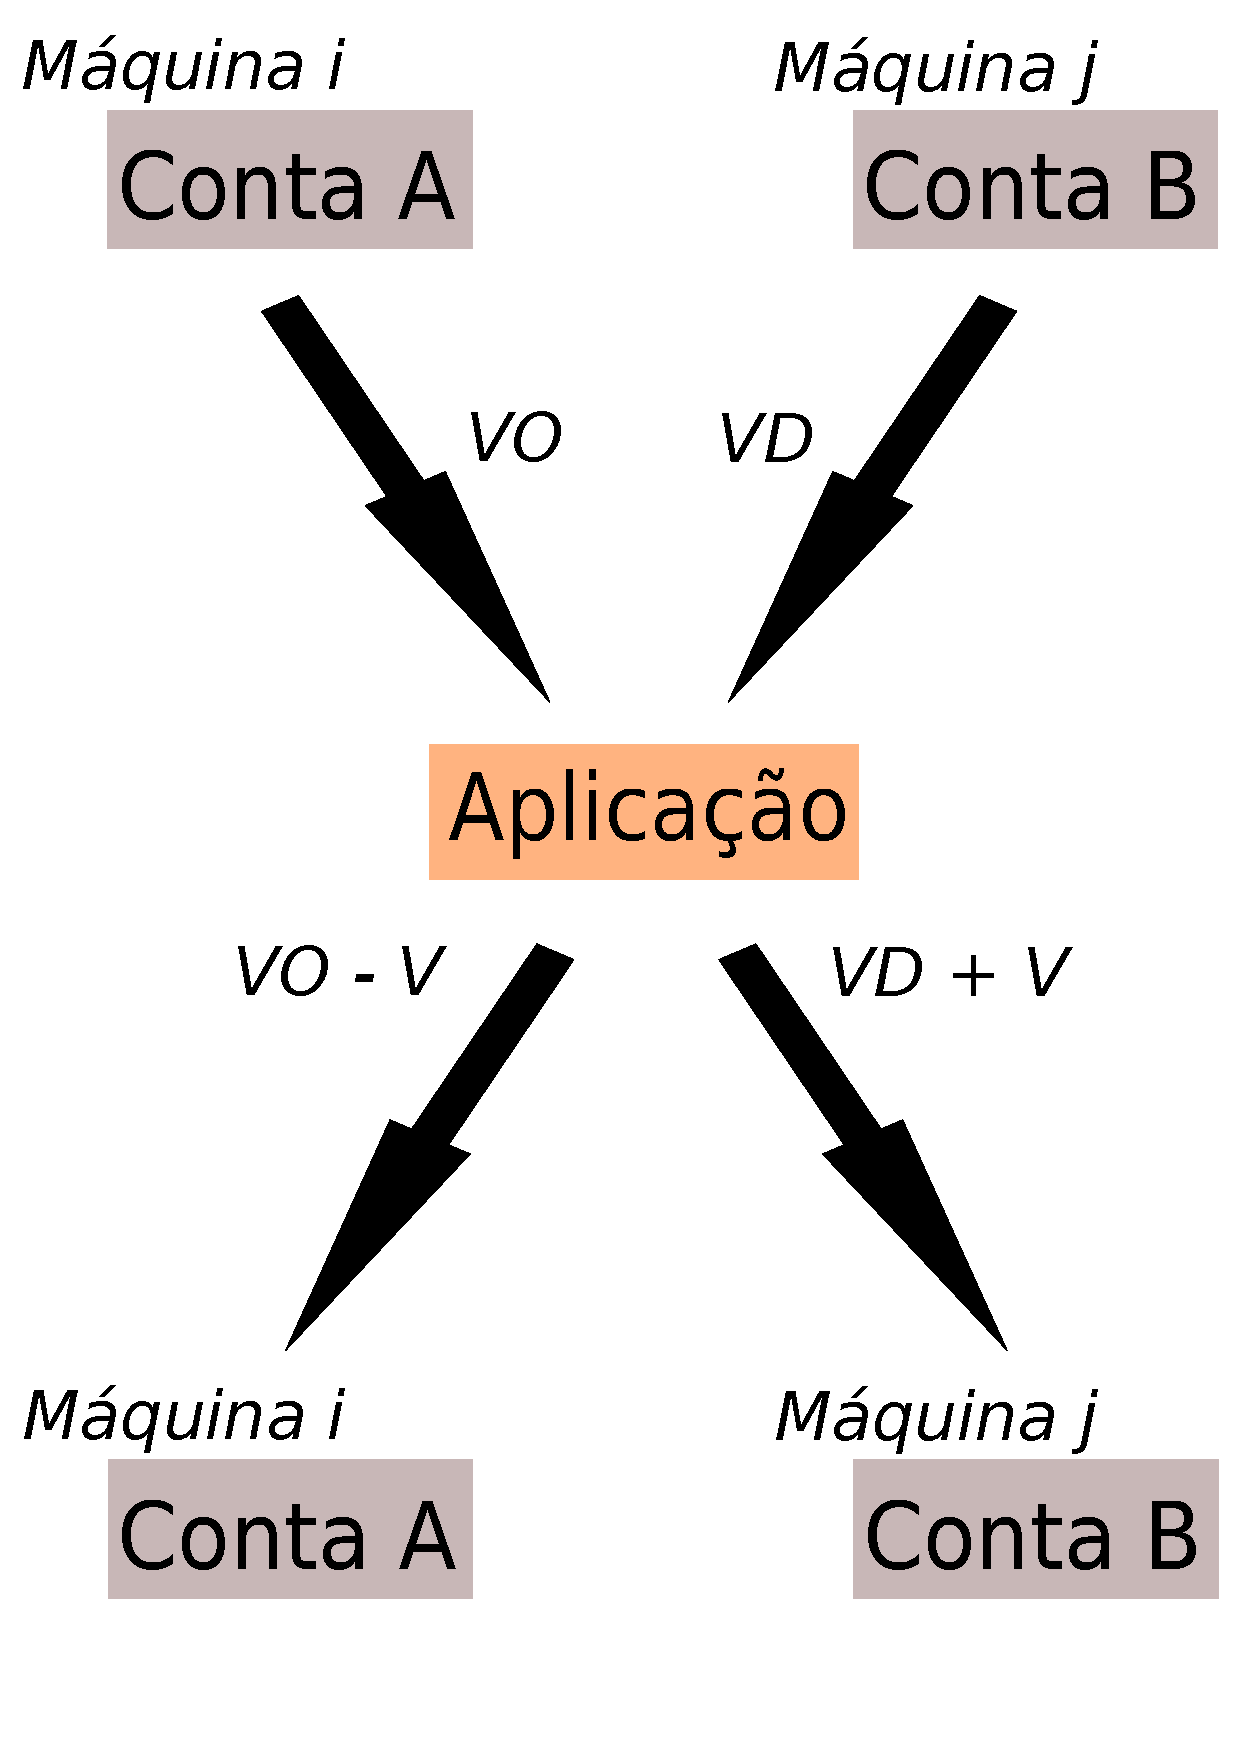
\includegraphics[width=.40\textwidth]{transacao_distribuida} 
  \caption{Esquematização de uma transação distribuída}
  \label{fig:transacao_distribuida} 
\end{figure}

%A atomicidade em um ambiente distribuído é mais difícil de se implementar do que em um ambiente centralizado devido aos novos erros que podem surgir, como falhas de comunicação ou de máquinas remotas. Por exemplo, digamos que a máquina i armazene a conta A e a máquina j armazene a conta B. 

Quando a aplicação inicia o procedimento que implementa o algoritmo para transferência entre contas, ela cria duas transações, uma na máquina i e outra na máquina j. A efetivação da transação na máquina i ocorre após a escrita na conta A e a efetivação na máquina j ocorre após a escrita na conta B. Se a máquina j não puder efetivar a sua transação, o sistema ficará inconsistente pois a transação na máquina i foi efetivada, ou seja, o valor foi subtraído da conta A.

Por isso, o controle de atomicidade em um banco de dados distribuído torna necessário algum mecanismo que permita que a transação seja bem sucedida somente se todas as subtransações forem bem sucedidas também, ou que a transação seja abortada caso alguma subtransação falhe. Este mecanismo é o protocolo de efetivação, que define uma série de passos a serem seguidos pelas máquinas executando as subtransações de forma que todas as máquinas envolvidas na transação concordem sobre a decisão de efetivar ou abortar a transação para que a atomicidade da transação seja garantida. O protocolo de efetivação mais usado é chamado de protocolo de efetivação de duas fases (\emph{Two-Phase Commit} --- 2PC), e ele será explicado na seção \ref{sec:2pc}.

%A recuperação de falhas em transações distribuídas também é complexa pois a qualquer momento uma máquina envolvida na transação pode falhar. É preciso ser garantido que quando a máquina que falhou voltar a operar a sua decisão em relação a efetivar ou abortar a transação seja consistente com a decisão global tomada para a transação. A recuperação de falhas está ligada à durabilidade da transação e está relacionada com a decisão de efetivar ou não a transação, e por isso também será ilustrado um mecanismo de recuperação de falhas na seção \ref{sec:2pc}.

Como descrito anteriormente na seção \ref{sec:transacoes}, uma maneira de efetuar controle de concorrência é através do uso de travas associadas aos dados acessados. Em um sistema não distribuído, o controle de alocação e liberação destas travas fica a cargo de um gerenciador de travas, um único componente que centraliza e sabe sobre todas as travas ativas no banco. Em um sistema distribuído, este gerenciamento de travas pode ser feito de várias maneira, variando desde de uma implementação totalmente centralizada, em que uma única máquina fica responsável por controlar os acessos, até uma implementação totalmente distribuída. A implementação centralizada é mais simples e direta, mas deixa o sistema vulnerável --- se a máquina escolhida para o gerenciamento de travas falhar, o sistema ficará indisponível. A abordagem totalmente distribuída torna o sistema mais independente e tolerante a falhas, mas aumenta a complexidade e a necessidade de comunicação entre as máquinas.

\section{Protocolo de efetivação de duas fases}
\label{sec:2pc}
A idéia deste protocolo é simples e utilizada a bastante tempo \cite{2pc}: verificar se todas as máquinas envolvidas em uma transação estão aptas a efetivar suas respectivas subtransações. Se estiverem, a transação será efetivada. Se algum participante não puder efetivar, por qualquer motivo, a transação será abortada. Neste protocolo existe o \textbf{coordenador}, uma máquina responsável por gerenciar a execução do protocolo e tomar a decisão sobre efetivar ou abortar a transação através da troca de mensagens com os \textbf{participantes}, as máquinas que executam as subtransações associadas à transação. O coordenador pode ser também um participante da transação.

Como seu nome diz, o protocolo é dividido em duas fases, ou rodadas. Na primeira fase o coordenador pede para que os participantes enviem seu voto para opinar se a transação pode ser efetivada ou não. Os votos são coletados e o coordenador avalia seus valores, decidindo se a transação pode ser efetivada (caso todos os participantes tenham votado de acordo) ou se deve ser abortada (caso algum participante tenha votado para não efetivar a transação). Decidido o resultado da votação, o coordenador efetua a segunda fase, em que os participantes são notificados do resultado da votação. Entre a execução da subtransação em cada participante e sua respectiva efetivação ou aborto, cada participante deve ser capaz de registrar as alterações efetuadas de forma permanente porém não definitiva, ou seja, de forma que possam ser desfeitas caso a transação seja abortada ou que possam ser aplicadas ao banco caso a transação seja efetivada. Neste contexto, os \emph{logs} dos participantes e do coordenador são de extrema importância no controle da transação distribuída e na garantia de sua atomicidade e durabilidade.

De forma mais detalhada, o protocolo de efetivação executa os algoritmos \ref{alg:2pc_coordenador}, \ref{alg:2pc_participante1} e \ref{alg:2pc_participante2} para efetivar uma transação $T$. O algoritmo \ref{alg:2pc_coordenador} descreve as ações do coordenador ao ser notificado que o protocolo deve iniciar. Os algoritmos \ref{alg:2pc_participante1} e \ref{alg:2pc_participante2} descrevem como os passos executados pelos participantes ao receberem uma solicitação de votação (primeira fase) e o resultado da votação (segunda fase), respectivamente. A função $Adicionar$ representa a operação de adicionar um elemento ao final do \emph{log}. A função $Enviar(d, m)$ representa o envio de uma mensagem $m$ para um destinatário $d$, e a função $Receber(r)$ representa o recebimento de uma mensagem de um remetente $r$. Uma visualização da execução do algoritmo pode ser vista nas figuras \ref{fig:2PC_1fase} e \ref{fig:2PC_2fase}.

\begin{algorithm}
\caption{Coordenador 2PC}
\label{alg:2pc_coordenador}
\begin{algorithmic}[1]
\State $Adicionar(log_c, (PREPARAR, T))$
\ForAll{$p_i \in Participantes$}
	\State $Enviar(p_i, (PREPARAR, T))$
\EndFor
\State $d \gets EFETIVAR$
\ForAll{$p_i \in Participantes$}
	\State $v \gets Receber(p_i)$
	\If{$v = ABORTAR$}
		\State $d \gets ABORTAR$
	\EndIf
\EndFor
\State $Adicionar(log_c, (d, T))$
\ForAll{$p_i \in Participantes$}
	\State $Enviar(p_i, (d, T))$
\EndFor
\end{algorithmic}
\end{algorithm}

\begin{algorithm}
\caption{Votação 2PC - $p_i$ recebe $(PREPARAR, T)$ de $c$}
\label{alg:2pc_participante1}
\begin{algorithmic}[1]
\State $v \gets Decidir(T)$
\State $Adicionar(log_i, (v, T))$
\State $Enviar(c, v)$
\end{algorithmic}
\end{algorithm}

\begin{algorithm}
\caption{Notificação 2PC - $p_i$ recebe $(d, T)$ de $c$}
\label{alg:2pc_participante2}
\begin{algorithmic}[1]
\If{$d = EFETIVAR$}
	\State $Efetivar(T)$
	\State $Adicionar(log_i, (EFETIVAR, T))$
\Else
	\State $Abortar(T)$
	\State $Adicionar(log_i, (ABORTAR, T))$
\EndIf
\end{algorithmic}
\end{algorithm}

A premissa que norteia o protocolo é que qualquer máquina envolvida na transação pode decidir abortá-la de forma unilateral, exigindo assim unanimidade na decisão pela efetivação da transação. As mensagens enviadas durante a execução do protocolo indicam uma decisão do remetente, e para garantir que essa decisão sobreviva a falhas na máquina que enviou a mensagem, os dados do \emph{log} são gravados em um meio de armazenamento estável, como um disco rígido, antes da mensagem ser enviada.

A transação $T$ é considerada oficialmente efetivada (ou abortada) no momento que o registro de $(EFETIVAR, T)$ (ou $(ABORTAR, T)$) do \emph{log} do coordenador for escrito para a área de armazenamento estável da máquina. Falhas posteriores não podem mudar a decisão do coordenador registrada em seu \emph{log} e gravada em disco.

\begin{figure}
  \centering
  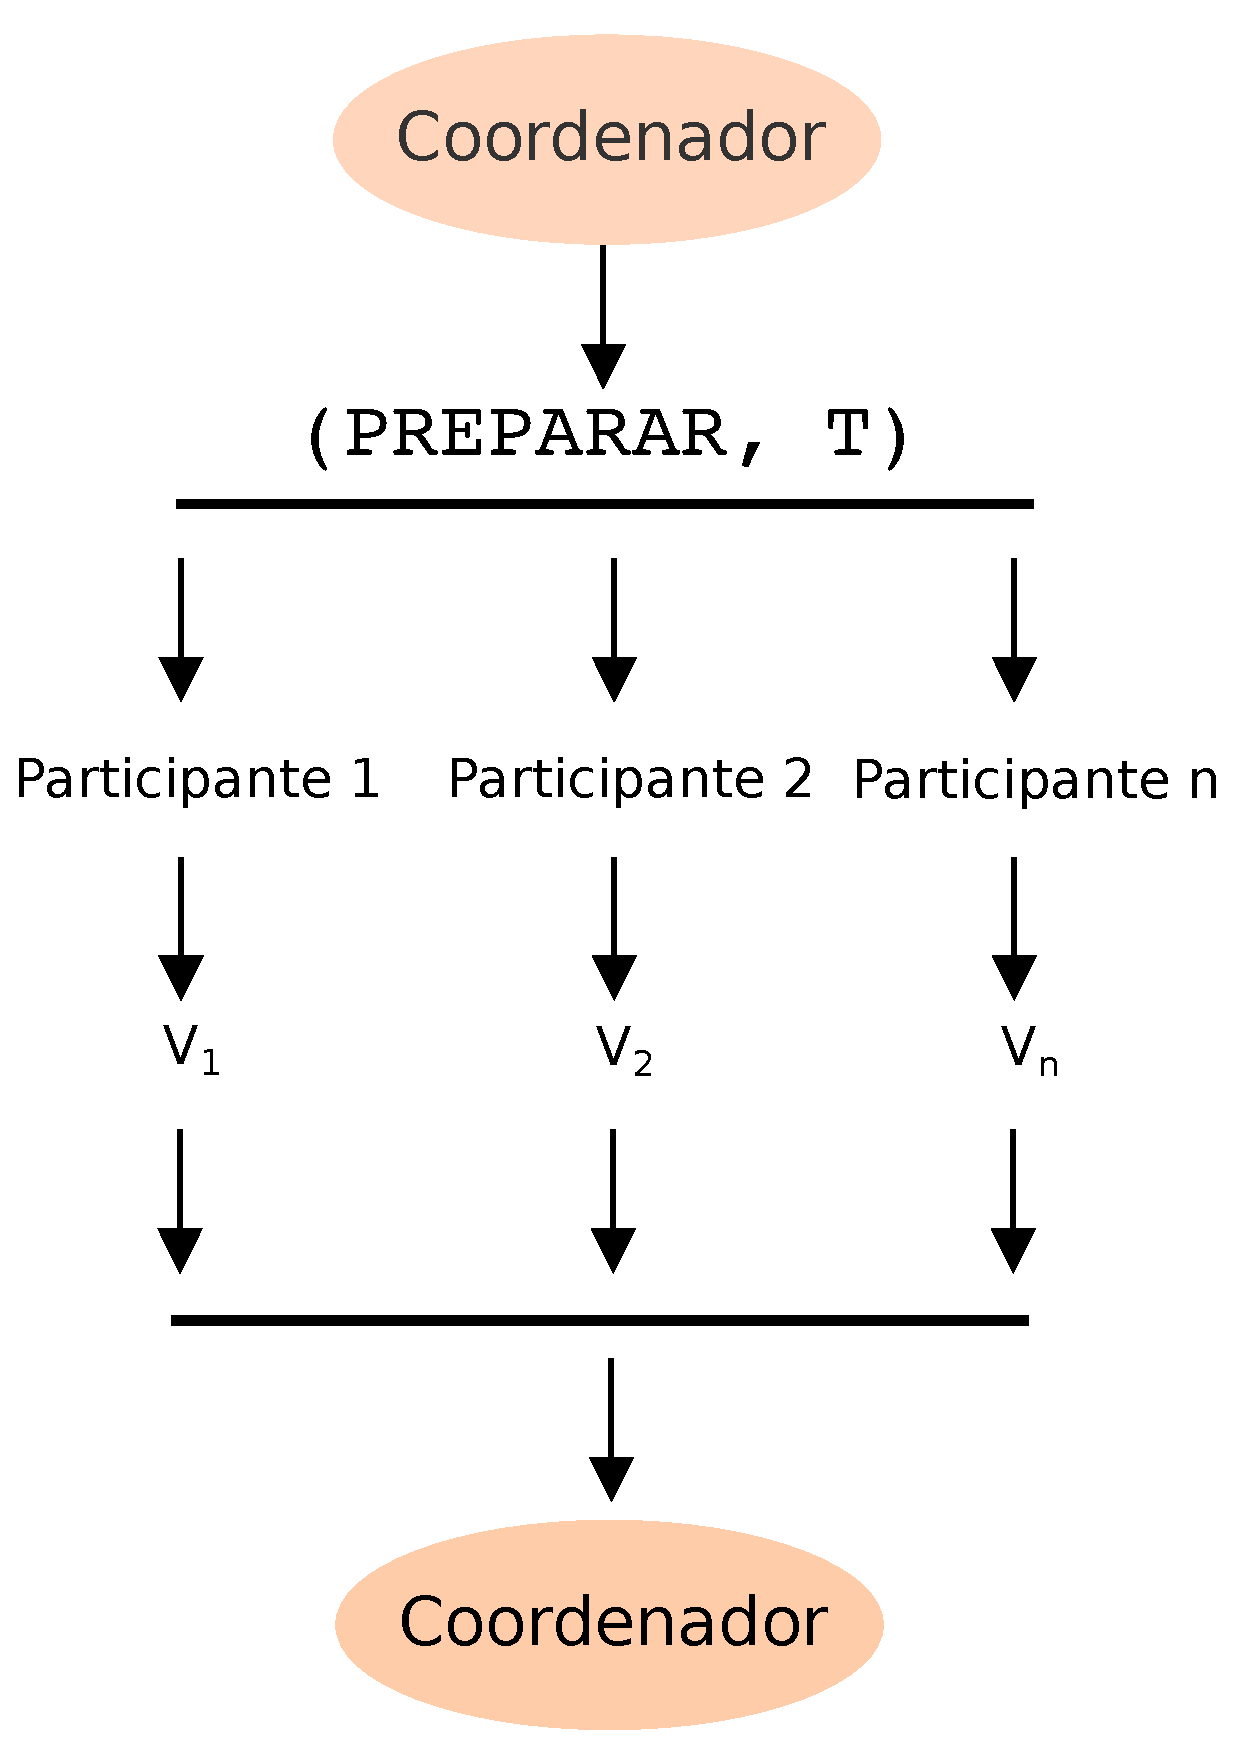
\includegraphics[width=.40\textwidth]{2PC_1fase} 
  \caption{Primeira fase - coordenador inicia a votação e os participantes respondem com seus votos $V_i$}
  \label{fig:2PC_1fase} 
\end{figure}

\begin{figure}
  \centering
  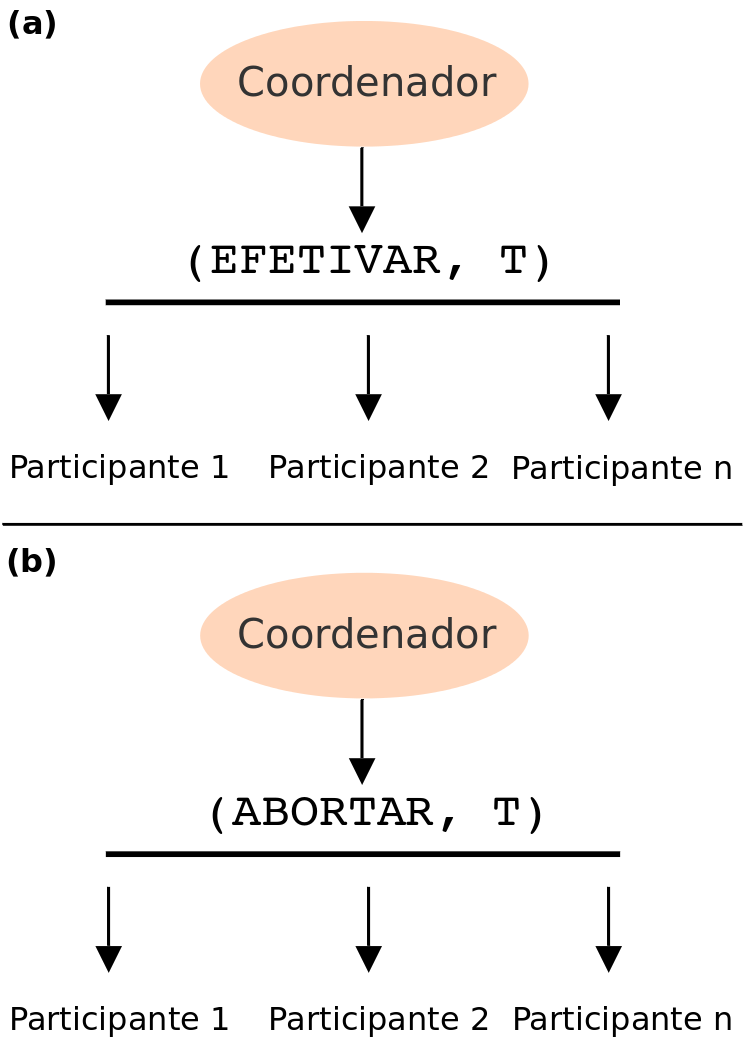
\includegraphics[width=.40\textwidth]{2PC_2fase} 
  \caption{Segunda fase - coordenador apura os votos e notifica os participantes. Em (a) os participantes são notificados de uma efetivação. Em (b), a transação foi abortada.}
  \label{fig:2PC_2fase} 
\end{figure}

É importante notar que este protocolo não define como as operações da transação devem ser executadas nas máquinas participantes, mas sim como a efetivação da transação deve proceder. As operações da transação devem ser todas enviadas para cada participante antes que o protocolo de efetivação inicie. Portanto, a execução deste protocolo aumenta o número de mensagens e consequentemente o tempo e o esforço necessários para que uma transação seja executada. Algumas otimizações podem ocorrer, como no caso de transações que efetuam somente operações de leitura ou de transações que envolvam dados em somente uma máquina do sistema mas, de forma geral, a execução do protocolo de efetivação de duas fases é custoso \cite{gray-lamport}.

\section{Minitransações}
\label{sec:minitransacoes}
As minitransações podem ser vistas como uma otimização do protocolo de efetivação de duas fases descrito em \ref{sec:2pc} em relação ao número de mensagens utilizadas. Elas constituem um mecanismo simples para ler e alterar dados em um ambiente distribuído garantindo atomicidade, consistência, isolamento e durabilidade \cite{sinfonia}. Porém, este ganho com a redução do número de mensagens utilizadas é obtido através da imposição de certas restrições em relação ao que pode ser feito com uma minitransação, diminuindo sua aplicabilidade.

Em \ref{subsec:derivando-minitransacoes} é apresentado como o protocolo 2PC pode ser usado como ponto de partida para otimizações e para a obtenção do protocolo de minitransações e em \ref{subsec:estrutura-minitransacoes} é descrita a estrutura e o protocolo de execução de uma minitransação.

\subsection{Otimização do 2PC}
\label{subsec:derivando-minitransacoes}
A decisão pela efetivação ou cancelamento de uma transação distribuída depende tanto de aspectos operacionais, relacionados ao ambiente de execução, quanto de aspectos semânticos, específicos do domínio da aplicação. A falha na execução de uma subtransação em alguma máquina do ambiente inviabiliza a efetivação da transação como um todo, e por isso o coordenador é forçado a cancelar a transação. Este tipo de falha operacional não está ligada ao domínio da aplicação, mas sim ao ambiente em que esta aplicação está rodando e está, portanto, fora do controle do coordenador, que pode somente cancelar a transação e, opcionalmente, tentar executá-la novamente. Por outro lado, o aspecto semântico envolvido na decisão pela efetivação ou cancelamento da transação é específico de cada aplicação e depende, direta ou indiretamente, dos dados do sistema.

Considerando novamente o sistema bancário e a operação de transferência de uma determinada quantia entre uma conta de origem e de destino, a transferência só pode ocorrer se o saldo na conta de origem da transferência for maior ou igual à quantia a ser transferida. Esse checagem deve ser feita pela aplicação após a leitura da informação da máquina que armazena os dados da conta de origem, e a decisão pelo cancelamento ou não da transação fica subordinado à semântica dada aos dados do sistema. Isso exige que uma requisição de leitura seja feita e uma resposta seja enviada, para só então a aplicação decidir se vai efetivar e então, após a execução do restante da transação, iniciar a primeira fase do protocolo 2PC (votação).

Portanto, podemos ver que do ponto de vista semântico as operações que influenciam na decisão pela possível efetivação ou pelo cancelamento da transação são operações de leitura. As operações de escrita não influenciam nessa decisão, a não ser pelo ponto de vista operacional, ou seja, se ocorrer realmente um erro na operação de escrita. Assim, se tivermos uma transação cuja última ação não afete a decisão do coordenador sobre efetivar a transação, podemos embutir esta última ação na mensagem de votação da primeira fase do protocolo, economizando uma mensagem.

O aspecto semântico da transação em relação aos dados pode ser tratado nos participantes, e não somente no coordenador, caso o participante saiba como o coordenador irá utilizar o dado para fazer sua decisão sobre efetivar ou cancelar a transação. Se isso for possível, podemos então embutir também operações de leitura que influenciam a decisão do coordenador no protocolo de efetivação e fazer o participante adequar seu voto à maneira como o coordenador faria ao analisar o dado retornado.

As minitransações surgem no contexto em que todas as operações de uma subtransação podem ser embutidas dentro do protocolo de efetivação, utilizando somente as trocas de mensagens que ocorreriam no protocolo de efetivação, após a execução dos comandos. Para que isso possa ocorrer, as mensagens do protocolo 2PC precisam ser alteradas para incluir informações sobre os dados a serem comparados, como veremos na próxima seção.

\subsection{Estrutura e protocolo}
\label{subsec:estrutura-minitransacoes}
Uma minitransação consiste de três conjuntos: itens de comparação, itens de leitura e itens de escrita, como pode ser visto na figura \ref{fig:estrutura_minitransacao}. Todos os itens possuem uma referência a qual dado deve ser utilizado, e os itens de comparação e escrita incluem também dados, que serão comparadas com ou substituirão os dados armazenados, respectivamente. 

\begin{figure}
  \centering
  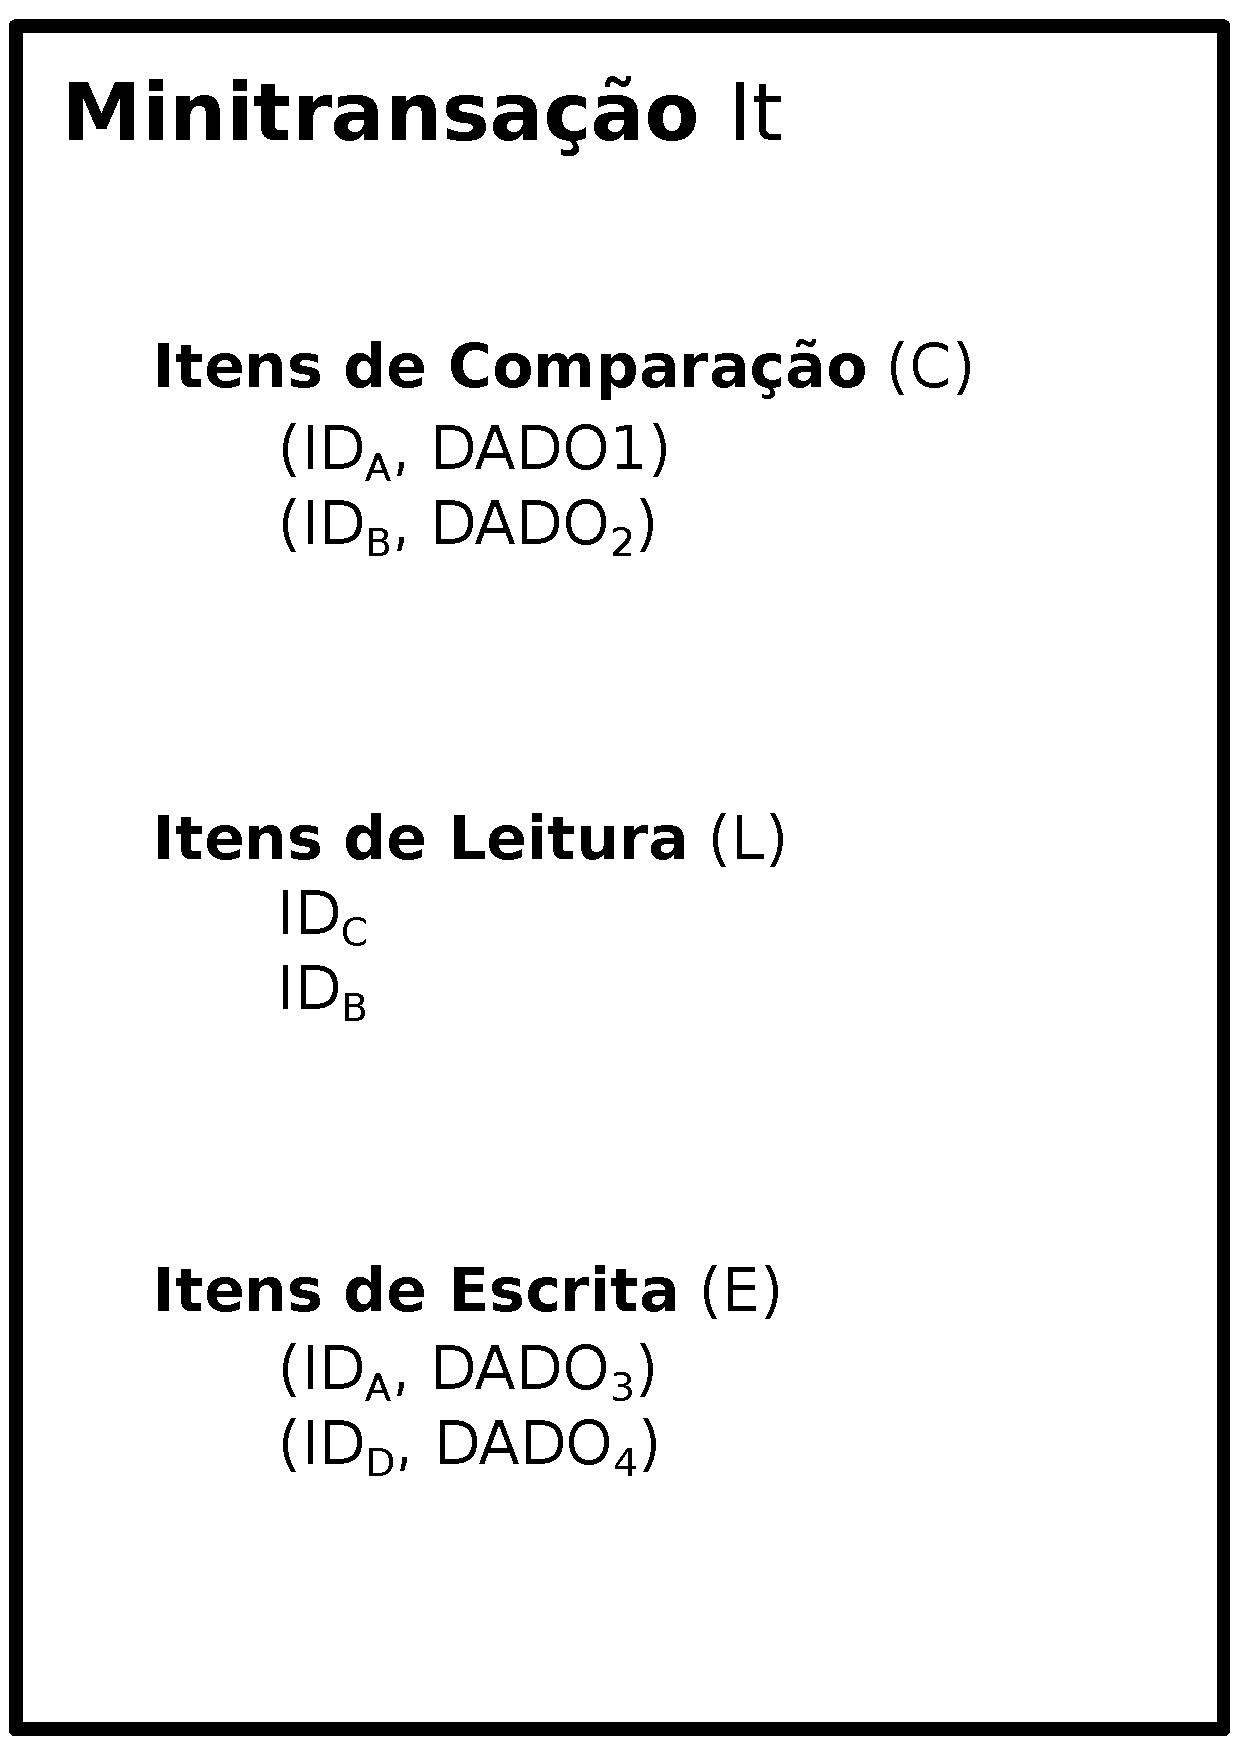
\includegraphics[width=.40\textwidth]{estrutura_minitransacao} 
  \caption{Estrutura de uma minitransação}
  \label{fig:estrutura_minitransacao} 
\end{figure}

Formalmente, uma minitransação pode ser vista como uma tupla na forma $(I_t, C, L, E)$. $I_t$ é o identificador da minitransação, permitindo aos participantes diferenciar e tratar minitransações simultâneas. \(C\) é o conjunto de itens de comparação, \(L\) é o conjunto de itens para leitura e \(E\) é o conjunto de itens para escrita. Os elementos de \(L\) são identificadores de dados, e o domínio de seus valores é o conjunto de identificadores armazenados na máquina participante. \(C\) e \(E\) possuem elementos que podem ser representados como tuplas no formato \((Id, Dado)\), em que \(Id\) é o identificador do dado e \(Dado\) é o valor para se comparar com o valor identificado por $Id$ ou para substituí-lo.

Para cada máquina \(P_i\) podemos definir \(K_i\) como sendo o conjunto de identificadores de dados armazenados em \(P_i\). Para executar uma transação cujo identificador seja \(I_t\) o coordenador deve primeiro identificar os participantes \(P_j\) da transação para quem as minitransações serão enviadas. Estes participantes são identificados através dos identificadores dos dados que a minitransação utiliza.

Para cada \(P_j\) é construída uma minitransação \(M_j = (I_t, C_j, L_j, E_j)\) tal que:

\begin{itemize}
\item $\forall i_l \in L_j, i_l \in K_j$;
\item $\forall i_c \in Id[C_j], i_c \in K_j$; e
\item $Id[E_j] \supseteq K_j$
\end{itemize}

Na notação acima $Id[X]$ representa o conjunto formado pelo elemento $Id$ de todas as tuplas no formato $(Id, Valor)$ do conjunto $X$. Os identificadores de $E_j$ são tratados como um superconjunto de $K_j$ pois a operação de escrita pode inserir novos dados no sistema, e não somente alterar dados que já existem.

Sendo uma extensão do \emph{2PC}, o protocolo de minitransações possui também um coordenador responsável por iniciar e gerenciar a execução do protocolo entre os participantes da transação. O protocolo de execução é composto também por duas fases, mas agora a primeira fase passa a ser uma fase de execução, em que as minitransações são enviadas para cada participante, que irá tentar executar as operações e responder com um voto de acordo com a situação. O coordenador coleta os votos de todos os participantes e, como no protocolo original, irá decidir por efetivar a transação somente se os votos forem unânimes. Na segunda fase os participantes são notificados da decisão do coordenador. O comportamento do coordenador e dos participantes é descrito pelos protocolos \ref{alg:mini_coordenador}, \ref{alg:mini_participante1} e \ref{alg:mini_participante2}.

O algoritmo \ref{alg:mini_coordenador} inicia construindo as minitransações para cada participante no conjunto $Participantes$. Este conjunto é determinado a partir do conjunto de identificadores $L \cup Id[C] \cup Id[E]$ da transação. A forma como é feito o mapeamento entre os identificadores e os participantes será explicado no capítulo \ref{chap:implementacao}. As minitransações são enviadas para cada participante $p_j \in Participantes$. O coordenador irá esperar pela execução e resposta de cada participante, que irão executar o algoritmo descrito em \ref{alg:mini_participante1}. Ao receber uma minitransação, cada participante irá tentar ler os dados identificados por $Id[C_j]$ e compará-los com os respectivos $Dado[C_j]$. Caso a comparação não seja bem sucedida, o participante votará então por abortar a transação, indicando isso em sua resposta, e nem tentará ler ou modificar os dados em $L_j$ e $E_j$.

Se a comparação for bem sucedida para todos os elementos de $Id[C_j]$, então o participante irá ler os dados identificados por $L_J$ e agrupá-los no conjunto $R_l$. Os dados $Dado[E_j]$ identificados por $Id[E_j]$ serão armazenados no \emph{log} do participante. O participante envia então a sua resposta para o coordenador. Ao coletar todas as resposta, o coordenador irá apurar os votos de cada participante. Para cada resposta $EFETIVAR$ há um conjunto, possivelmente vazio, de elementos lidos. O algoritmo \ref{alg:mini_coordenador} agrega todos esses conjuntos para as minitransações que votaram por efetivar a transação em um conjunto $R$ e utiliza esse conjunto para executar a lógica específica do domínio da aplicação e decidir, de acordo com critérios semânticos, se a transação irá ser efetivada ou não ($d \gets Decidir(R)$). A decisão sobre efetivação ou não da transação é então comunicada a cada participante, que irá executar o algoritmo \ref{alg:mini_participante2} para finalmente efetivar as operações que a mini-transação executou ($Efetivar(I_t)$) ou para abortá-las ($Abortar(I_t)$). $Efetivar(I_t)$ irá vasculhar o \emph{log} de operações para aplicar as operações aos dados, e $Abortar(I_t)$ irá ignorar as operações dos mesmos.

Notamos que, de forma contrária ao que ocorre no \emph{2PC}, o coordenador nunca escreve em um \emph{log}. Neste protocolo somente os participantes utilizam o \emph{log}, e o protocolo não fica paralizado caso o coordenador falhe. O protocolo só não terá progresso se algum participante que está processando a transação falhar, pois neste ponto o coordenador não saberá o que fazer. O processo de recuperação de falhas e monitoração será explicado no capítulo \ref{chap:implementacao}.

\begin{algorithm}
\caption{Coordenador - recebe um transação no formato $(I_t, C, L, E)$}
\label{alg:mini_coordenador}
\begin{algorithmic}[1]
\ForAll{$p_j \in Participantes$}
	\State $Enviar(p_j, (I_t, C_j, L_j, E_j))$
\EndFor
\State $d \gets EFETIVAR$
\State $R \gets \{\}$
\ForAll{$p_j \in Participantes$}
	\State $(v_j, r_j) \gets Receber(p_j)$
	\If{$v_j = ABORTAR$}
		\State $d \gets ABORTAR$
	\Else
		\State $R \gets r_j \cup R$
	\EndIf
\EndFor
\If{$d \neq ABORTAR$}
	\State $d \gets Decidir(R)$
\EndIf
\ForAll{$p_j \in Participantes$}
	\State $Enviar(p_j, (d, I_t))$
\EndFor
\end{algorithmic}
\end{algorithm}

\begin{algorithm}
\caption{Execução - $p_j$ recebe $(I_t, C_j, L_j, E_j)$ de $c$}
\label{alg:mini_participante1}
\begin{algorithmic}[1]
\State $d \gets EFETIVAR$
\ForAll{$c \in C_j$}
	\If{$Dado(c) \neq Ler(Id(c))$}
		\State $d \gets ABORTAR$
	\EndIf
\EndFor
\State $R_l \gets \{\}$
\If{$d = EFETIVAR$}
	\ForAll{$l \in L_j$}
		\State $R_l \gets Ler(Id(l)) \cup R_l$
	\EndFor
	
	\ForAll{$e \in E_j$}
		\State $Adicionar(log_{p_j}, ( (Id(e), Dado(e)), I_t ) )$
		%\State $Escrever(Id(e), Dado(e))$
	\EndFor
\EndIf
\State $Enviar(c, (d, R_l))$
\end{algorithmic}
\end{algorithm}

\begin{algorithm}
\caption{Confirmação - $p_j$ recebe $(d, I_t)$ de $c$}
\label{alg:mini_participante2}
\begin{algorithmic}[1]
\If{$d = EFETIVAR$}
	\State $Efetivar(I_t)$
\Else
	\State $Abortar(I_t)$
\EndIf
\end{algorithmic}
\end{algorithm}

\section{Trabalhos relacionados}
\label{sec:trabalhos_relacionados}
O conceito de minitransações é introduzido como base para a construção de \emph{Sinfonia} (\cite{sinfonia}), que é um sistema cujo foco é prover a base para o desenvolvimento de sistemas distribuídos de baixo nível, como sistemas de arquivos distribuídos, gerenciadores de travas ou serviços de comunicação de grupos de computadores, enquanto que o objetivo deste trabalho é utilizar as minitransações como base para a construção de uma infraestrutura que facilite o desenvolvimento de aplicações distribuídas de alto nível, como sistemas de comércio eletrônico ou redes sociais. 

\emph{Sinfonia} é composto por nós de memória mas a interface exposta por estes componentes é diferente: cada nó de memória mantém uma sequência de bytes puros, sem dar interpretação específica a esses bytes. Estes bytes são organizados como em um espaço de endereçamento linear, sem nenhuma estrutura. Cada nó de memória possui um espaço de endereçamento separado de forma que os dados são referenciados por um par que especifica o nó de memória e o endereço deste dado. Em nossa infraestrutura, o acesso é feito através de uma única chave, que é um conjunto de bytes que faça sentido para a aplicação.

Ao invés de utilizar um componente de acesso como em nossa infraestrutura, \emph{Sinfonia} disponibiliza uma biblioteca que é compilada junto ao aplicativo cliente, e o acesso aos nós de memória são efetuados por esta biblioteca. Em nosso infraestrutura, o componente de acesso permite isolar a aplicação de detalhes da distribuição dos dados entre os nós de memória, e pode ser acessado pela rede através do protocolo TCP/IP. Acreditamos que esta abordagem seja mais efetiva que a abordagem que utiliza uma biblioteca, pois qualquer linguagem que permita o comunicação TCP/IP poderá utilizar nossa infraestrutura, ao passo que se disponibilizarmos uma biblioteca, somente as linguagens para as quais uma biblioteca for escrita poderão usufruir da infraestrutra.

\cite{padilha} apresenta um sistema de armazenamento baseado em minitransações tolerante a falhas bizantinas. Em sistemas que toleram somente componentes com falhas simples (\emph{fail-stop components}), é assumido que um componente pode estar em dois estados: ativo e inativo. Se estiver em um estado ativo, o componente se comportará de acordo com a especificação do sistema. Se estiver inativo, o componente simplesmente para de interagir com o sistema. Está é uma simples e um tanto simplificada de lidar com falhas no sistema, mas é a forma utilizada por diversos sistemas, entre ele \emph{Sinfonia} e a nossa infraestrutura. A maneira mais geral de lidar com falhas é através de falhas bizantinas (\cite{byzantine}). Em sistemas que lidam com este tipo de falha, um componente ativo pode se comportar de forma incorreta, enviando mensagens errada ou mesmo mensagens sem sentido. O tratamento de falhas bizantinas não será discutido neste trabalho.

Existem diversos sistemas que visam o armazenamento escalável de informações e a disponibilização de serviços para facilitar o desenvolvimento de sistemas distribuídos, em geral tendo em vista a utilização para prover serviços a aplicações de internet de larga escala. Entre eles, podemos citar Bigtable (\cite{bigtable}), Dynamo (\cite{dynamo}), ZooKeeper (\cite{zookeeper}), PNUTS (\cite{pnuts}), entre outros. Bigtable é o sistema que permite ao Google armazenar de forma eficiente grandes quantidades de dados, provendo um tipo de consistência chamada de eventual (\cite{eventual_consistency}), assim como o Dynamo, da Amazon. Este tipo de consistência permite que dados sejam particionados e replicados para obter melhor performance e disponibilidade, mas permitem que diferentes máquinas possam ter versões diferentes de uma mesma informação. ZooKeeper é um sistema que provê serviços de coordenação e sincronização para a construção de sistemas distribuídos que utiliza o algoritmo Paxos (\cite{paxos}) para garantir consistência entre as operações. Como o foco do ZooKeeper é permitir a coordenação entre componentes de uma sistema distribuído, sua capacidade de armazenamento é limitada (em um megabyte), e portanto não é utilizável como um repositório de dados. PNUTS é o serviço de armazenamento de dados do Yahoo! que provê um tipo de consistência mais forte que a consistência eventual, porém mais fraca que a consistência obtida através de escalonamentos sequenciáveis de operações --- a chamada consistência na linha do tempo (\emph{timeline consistency}), em que todas as réplicas de um determinado objeto armazenado executam as mesmas alterações neste objeto na mesma ordem. Este sistema oferece também uma primitiva de acesso chamada \emph{test-and-set-write}, que efetua uma escrita de dados somente se uma comparação for bem sucedida, semelhante à forma de execução de nossa infraestrutura.

\chapter{Implementação}
\label{chap:implementacao}
Este capítulo irá apresentar a proposta de arquitetura e desenvolvimento da infraestrutura. A arquitetura e a interface de acesso serão discutidas na seção \ref{sec:arquitetura}. A seção \ref{sec:algoritmos} descreve as estruturas de dados e algoritmos utilizados para implementar a executação das minitransações e das operações relacionadas, como recuperação de falhas, controle de concorrência e persistência dos dados. A seção \ref{sec:aplicacoes} irá apresentar alguns exemplos de aplicações utilizando a infraestrutura desenvolvida e a última seção, \ref{sec:testes}, irá descrever o ambiente de testes, os testes realizados e os resultados obtidos.

\section{Arquitetura e interface}
\label{sec:arquitetura}

A infraestrutura desenvolvida neste trabalho é um sistema composto por componentes de armazenamento de dados e execução de minitransações e por componentes de acesso (o nome componente se refere à funcionalidade, e podemos ter mais de um componente em um máquina). O componente de armazenamento e execução é responsável por prover acesso aos dados sob sua responsabilidade através da execução das operações expecificadas nas minitransações, e é chamado de \emph{nó de memória}. O componente de acesso é o ponto de comunicação entre a aplicação e a infraestrutura, atuando como o coordenador das transações.

A figura \ref{fig:overview_arquitetura} ilustra de maneira simplificada a relação entre os componentes do sistema. O itens \emph{App} representam as aplicações que acessam a infraestrutura (eles não fazem parte da infraestrutura), os itens \emph{$C_a$} representam os componentes de acesso e os itens \emph{$C_e$} representam os nós de memória. Cada aplicação pode acessar qualquer componente de acesso que, como coordenadores, irão identificar os nós de memória participantes da transação e seguir o algoritmo \ref{alg:mini_coordenador}, não havendo uma estrutura rígida em relação à conexão dos componentes.

\begin{figure}
  \centering
  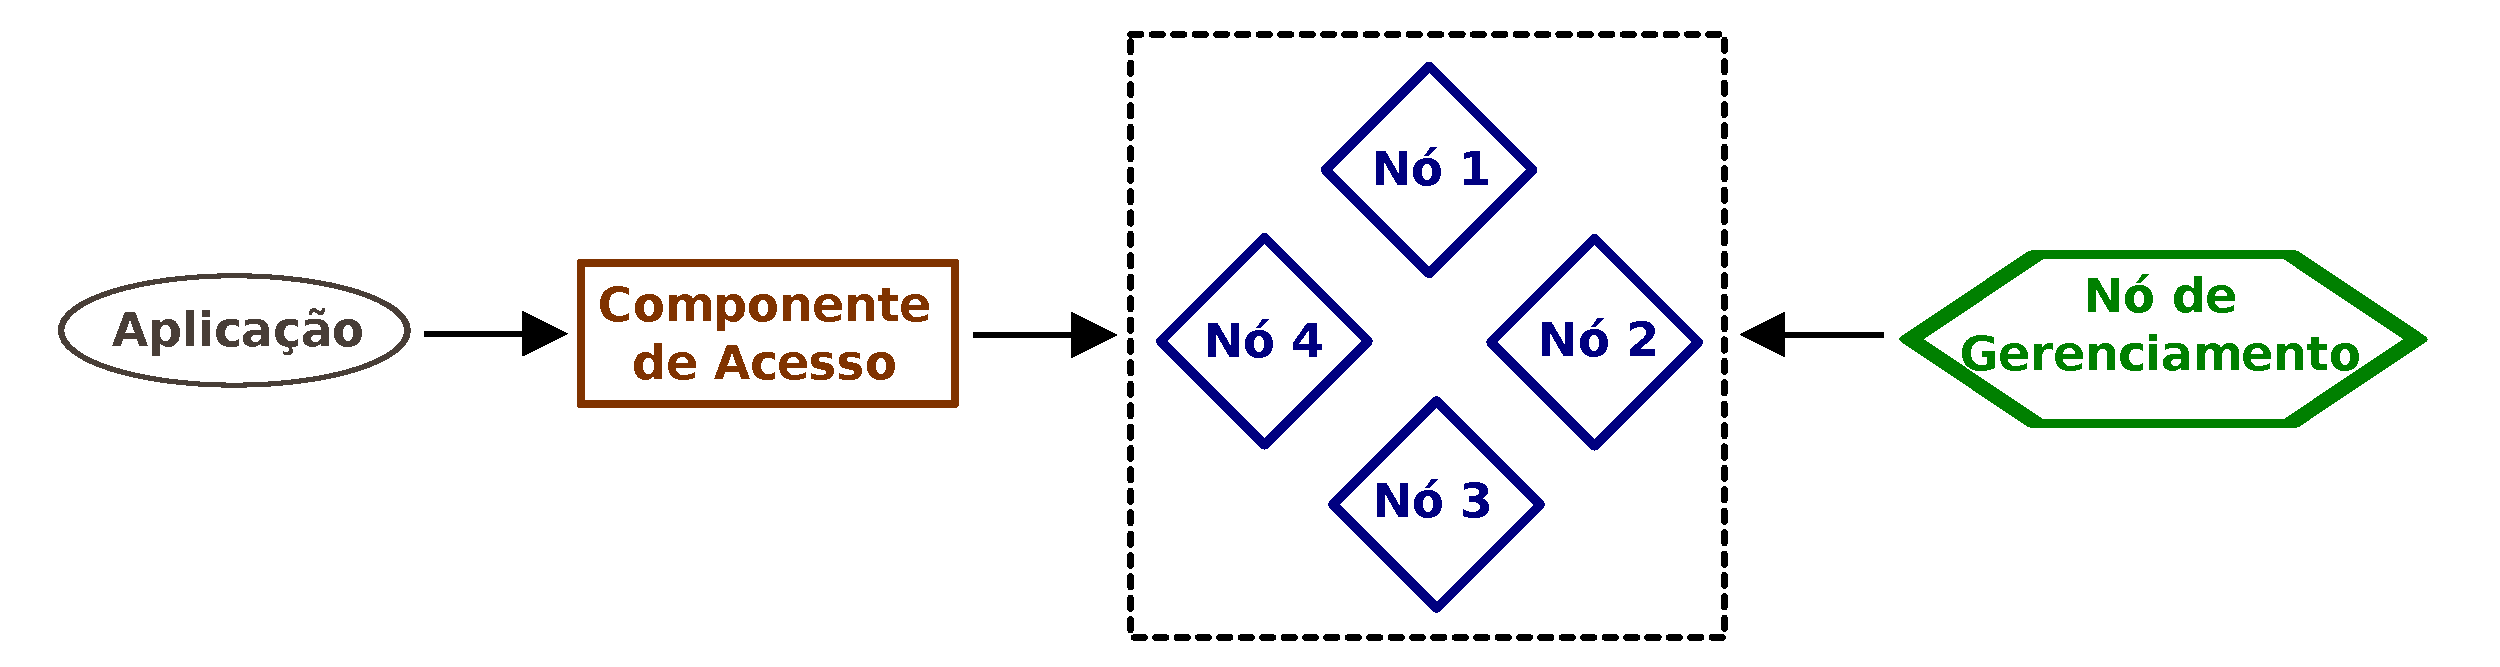
\includegraphics[width=.40\textwidth]{overview_arquitetura} 
  \caption{Visão geral da arquitetura da infraestrutura}
  \label{fig:overview_arquitetura} 
\end{figure}

A interface de acesso oferecida aos clientes da infraestrutura é a de uma tabela associativa chave-valor: os nós de memória armazenam um sequência de bytes (valor) nomeados por uma chave. Cada chave é única e o número de bytes utilizados para armazenar o valor é, teoricamente, ilimitado. 

\section{Algoritmos e estruturas de dados}
\label{sec:algoritmos}
Nesta seção serão descritos os algoritmos e as estruturas de dados principais para a execução das minitransações, para o controle de concorrência entre minitransações e para a recuperação de falhas do sistema. Os mecanismos aqui apresentados são baseados em métodos tradicionais de bancos de dados: travas para o controle de concorrência, como em bancos de dados com abordagem pessimista, e uso de um \emph{log} para controle de falhas e atomicidade.

O sistema está distribuído em $n$ máquinas $P_1, P_2, \dotsc, P_n$, e cada $P_i$ armazena um conjunto de informações $D_i$. O conjunto de dados $D = \bigcup_{i=1}^n D_i$ representa então o estado do sistema. Supondo a execução de uma minitransação com identificador \(I_t\), há três estruturas de dados principais utilizadas pelo sistema:
\begin{itemize}

\item \textbf{Tabela de dados}: Cada conjunto \(D_i\) é representado por uma tabela associativa, que pode ser visto como uma função que associa um identificador a um valor, representados respectivamente por \(Id(X)\) e \(Dado(X)\), onde \(X \in D_i\). Esta tabela suporta as operações \(Leitura(Id(X))\), que retorna \(Dado(X)\) ou um valor especial (\(NULO\)) caso \(X \notin D_i\), e \(Escrita(Id(X), V)\), que atribui a \(Dado(X)\) o valor \(V\) caso $X \in D_i$ ou  que insere $X$ em $D_i$ ($D_i \gets D_i \cup X$) caso contrário. 

\item \textbf{Tabela de travas}: Para controlar o acesso concorrente aos dados de \(D_i\) é utilizada também uma tabela associativa entre um identificador e uma trava. onde a trava é um valor do conjunto \(\{LEITURA, ESCRITA, LIVRE\}\). Assim, para \(X \in D_i, Trava(X) \rightarrow Y, Y \in \{LEITURA, ESCRITA, LIVRE\}\). Se \(Y\) for \(LIVRE\), isso indica que o identificador não possui nenhuma trava associada, e pode ser lido ou escrito sem problemas. Se \(Y\) for \(LEITURA\), isso quer dizer que somente leituras podem ocorrer no identificador associado e escritas estão proibidas. Se \(Y\) for \(ESCRITA\) então nem leituras nem escritas podem ocorrer no identificador associado. Esta tabela suporta as operações \(TentarTravar(I_t, X, T), T \in \{LEITURA, ESCRITA\}\), que verifica se a trava \(T\) pode ser associada ao identificador \(X\) pela transação \(I_t\) e retorna uma valor em $\{TRAVOU, NAO_TRAVOU\}$, \(Liberar(I_t, X)\), que retira a trava que \(I_t\) atribuiu a \(X\), e $Promover(I_t, X)$, que permite que a trava obtida pela transação $I_t$ para o identificador $X$ seja promovida de $LEITURA$ para $ESCRITA$, retornando um valor em $\{PROMOVEU, NAO_PROMOVEU\}$. Esta promoção só ocorre caso $I_t$ tenha obtido previamente uma trava $LEITURA$ e nenhuma outra transação tenha travas $LEITURA$ no mesmo dado $X$.

\item \textbf{Tabela de escrita temporária}: Esta tabela é estruturalmente idêntica à tabela de dados, mas seu objetivo é diferente. As escritas de um minitransação são efetuadas nesta tabela durante a execução da minitransação e, somente após a notificação da efetivação da minitransação é que o participante irá transferir os dados escritos desta tabela de escrita temporária para a tabela de dados. Esta estrutura suporta as mesmas operações que a tabela de dados.
\end{itemize}

A execução da transação \(I_t\) é efetuada de maneira distribuída entre o coordenador da transação e o participante. O comportamento do coordenador é descrito pelo algoritmo \ref{alg:mini_coordenador}. Diferentemente do \emph{2PC}, o protocolo de execução das minitransações não grava nenhum registro no \emph{log} do coordendaor. O coordenador envia uma minitransação no formato \(M = (I, C, L, E)\) para cada participante \(P_i\) da transação através do algoritmo \ref{alg:mini_coordenador}. $I$ é o identificador da transação, devendo ser único em todo o sistema. $C$ é o conjunto de itens de comparação, $L$ é o conjunto de itens a serem lidos e $E$ é o conjunto de dados a serem atualizados ou inseridos.

O algoritmo \ref{alg:mini_coordenador} inicialmente gera um identificador único para a transação a ser executada, $I_t$. Todas as máquinas do sistema que irão participar da transação são identificadas através do conjunto de identificadores dos dados dos conjuntos $C$ de itens de comparação, $L$ de leitura e $E$ de escrita da transação. O algoritmo então envia uma minitransação para cada participante com os respectivos itens de comparação, leitura e escrita de cada participante, identificando a transação com $I_t$. A resposta enviada pelo participante é armazenada para descobrirmos o resultado da transação. As linhas 2---10 representam a primeira fase do protocolo, equivalente à fase de votação do \emph{2PC}.

As linhas 11---18 ilustram a segunda fase do protocolo. Se todos os participantes votaram $SIM$ (o conjunto de votos é obtido do conjunto de respostas $R$ através de $Voto(R)$) e a aplicação decidiu efetivar a transação ($Processar(Dado(R))$ representa a lógica específica da aplicação que utiliza os dados obtidos do conjunto de respostas através de $Dado(R)$), então a transação será efetivada, representado por $resultado \gets EFETIVAR$. Caso contrário, a transação será abortada. Esse resultado é então enviado para os participantes, e o protocolo termina.

\section{Aplicações desenvolvidas utilizando a infraestrutura}
\label{sec:aplicacoes}
A ser definido...

\section{Execução dos testes}
\label{sec:testes}
A ser definido...

\chapter{Cronograma}
\label{chap:cronograma}
Os próximos passos no trabalho serão:

\begin{itemize}
\item Desenvolvimento da infraestrutura: deverão ser implementados os nós de memória e os componentes de acesso, efetuando controle simples de concorrência (através de travas associadas aos identificadores acessados) e de recuperação de erros. Período: Julho/2012 - Outubro/2012.
\item Desenvolvimento das aplicações de teste: aplicações simples que permitam explorar e analisar a utilização e a performance da infraestrutura. Período: Outubro/2012 - Dezembro/2012.
\item Testes das aplicações: execução dos testes, coleta e análise dos dados obtidos. Período: Janeiro/2013 - Abril/2013.
\end{itemize}

% cabeçalho para os apêndices
\renewcommand{\chaptermark}[1]{\markboth{\MakeUppercase{\appendixname\ \thechapter}} {\MakeUppercase{#1}} }
\fancyhead[RE,LO]{}
\appendix

%\include{apendice} 

% ---------------------------------------------------------------------------- %
\backmatter \singlespacing   % espaçamento simples
\bibliographystyle{alpha-ime}% citação bibliográfica alpha
\bibliography{bibliografia}  % associado ao arquivo: 'bibliografia.bib'

% ---------------------------------------------------------------------------- %
% Índice remissivo
%\index{TBP|see{periodicidade região codificante}}
%\index{DSP|see{processamento digital de sinais}}
%\index{STFT|see{transformada de Fourier de tempo reduzido}}
%\index{DFT|see{transformada discreta de Fourier}}
%\index{Fourier!transformada|see{transformada de Fourier}}
%\printindex   % imprime o índice remissivo no documento 

\end{document}
